\chapter{Materials and Methods}
\label{chap:methods}
%\pagenumbering{arabic}

In this chapter we describe the model implemented on a robot for learning of sensorimotor competences at early stages of development in children. 
We start by explaining the development of hand-eye coordination in \ref{sec:hecoord}, an important motor skill that develops early in infancy. We proceed by explaining the body babbling (mentioned in section \ref{sec:devsoccog}) algorithm  implemented on a robot. Then, we introduce the biologically inspired model based on self-organising maps in section \ref{sec:themodel}. We explain the biological motivation, the model architecture and implementation details. Finally, in section \ref{sec:modeltrain} we explain how data acquired through random body babbling is used to tune the model.

\section{Hand-Eye Coordination}
\label{sec:hecoord}

Control of limbs is one of the first motor skills which humans learn.
Hand-eye coordination is acquired early in infancy where visual input is used to control, guide and direct hand movements. 
Vision in infants develops gradually and is largely dependent upon the bodily experience \citep{pmid9455172}. For example, infants at the age of 3 months exhibit saccadic movements only in the retinocentric reference. At the age of 3 or 4 months ``hand regard'' behaviour is observed when they are able to gaze at their own hands moving in front of their faces. At the age of 7 months they perform saccadic movements in the body-centered reference frame.
Visual guidance is thus essential for the development of gross and fine motor skills that are used in everyday interactions with the environment.
Ability to coordinate finger and arm movements, grasping, reaching, and the ability use hands to manipulate objects is known as \emph{dexterity}. 
Dexterity in artificial agents such as robots remains a difficult challenge due 
to several reasons. 
For example, depending on the number of degrees of freedom, there could 
be infinite many arm configurations that result in the same hand position. 
It is the task of a roboticist to determine what arm configurations are feasible and how to deal with the curse of dimensionality due to many degrees of freedom of the robot's arm. Another example is the problem of depth perception when using a single camera for visual input. Without depth information the robot is not able to point because of a similar reason - there are many different arm configuration resulting in the same perceived marker position (Figure \ref{lab:handpositions}). To address these problems we analyse learning mechanisms infants employ to acquire similar skills.
In the early stages of development infants gradually learn to acquire  sensorimotor coordination.
They learn configurations of arm postures through a set of self-exploration activities such as body babbling. 

\begin{figure}[h]
\centering
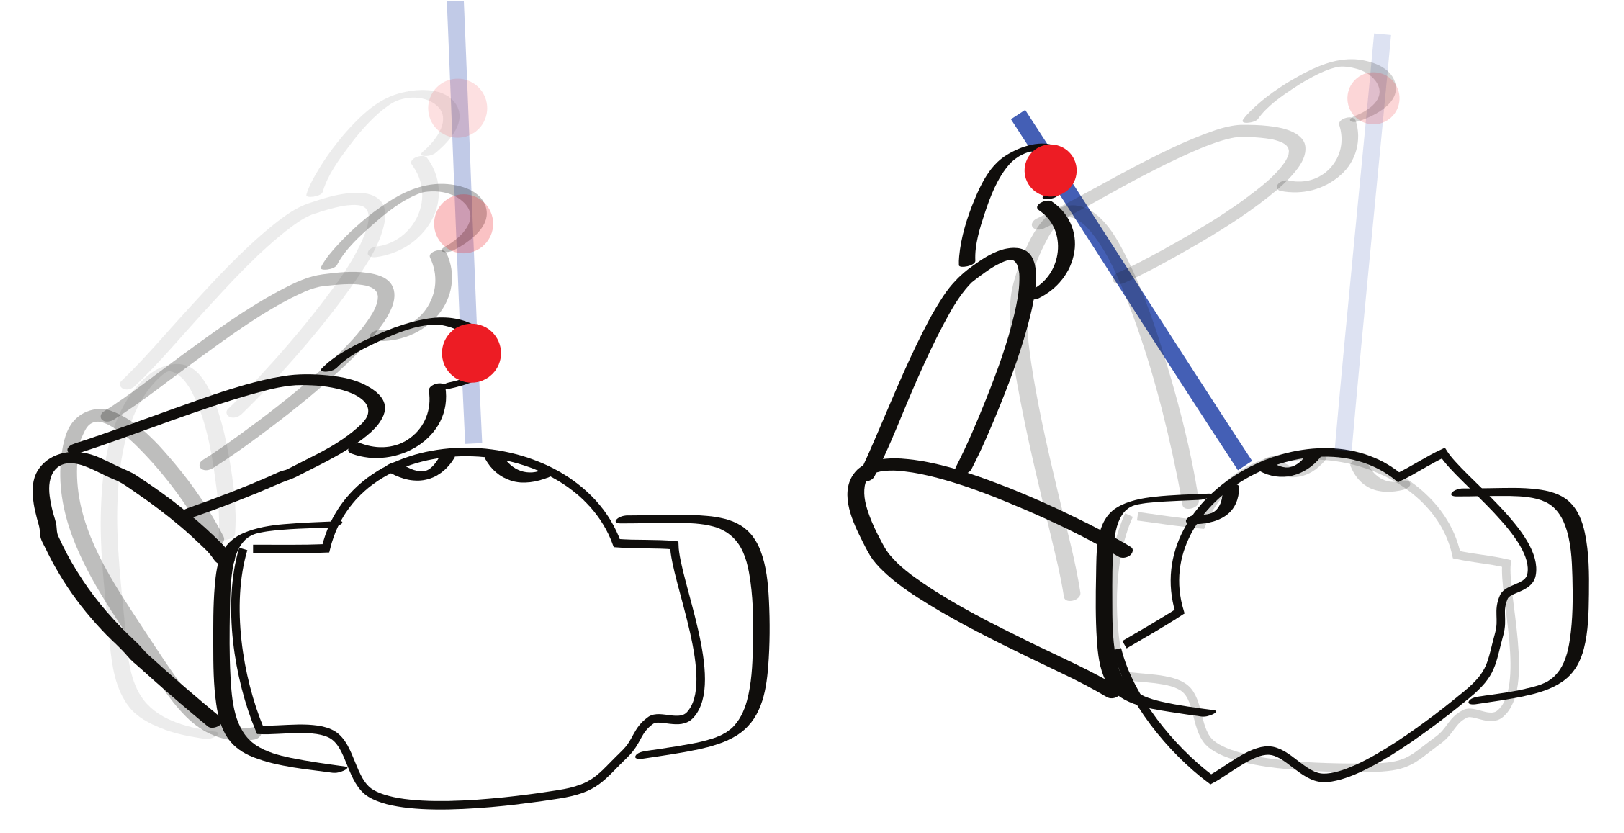
\epsfig{file=multiple_config.png, height=4cm}
\caption{Multiple arm configurations result in the same perceived marker position}
\label{lab:handpositions}
\end{figure}


\subsection{Random Motor Babbling}
\label{sec:babbling}

Body babbling employed by infants is motor experience for mapping movements to the resulting body configurations \citep{Meltzoff97}. 
To avoid exploring the whole set of possible arm configurations, infants 
constantly try to reach objects surrounding them even if that reaching results 
in failed actions. As explained in the chapter \ref{sec:devsoccog}, it is 
assumed that pointing emerges from such failed reaching actions which are 
interpreted as the infant's request for an object. 
%The idea that infants do not employ purely random babbling gestures underlies the theory of goal babbling.
Body babbling is fundamental in learning of limb postures and correlations between motor actions and resulting sensory input. In developmental robotics, body babbling can be used for the acquisition of basic motor competences such as hand-eye coordination \citep{Lungarella2003} that eventually lead to the development of more complex behaviours such as sharing of the attention through pointing \citep{Hafner2011}. 
There are several limitations to the random body babbling algorithm, such as inability to switch between exploration of new postures and exploitation of existing ones based on robot's learning interest. Goal directed behaviours have been proposed in \citep{olsson2006} and \citep{baranes2013}, showing that it is possible to gradually integrate information about the robot's sensory system in a developmental paradigm. However, the scope of this thesis does not deal with such advanced exploration behaviours.

\begin{figure}[t]
\centering
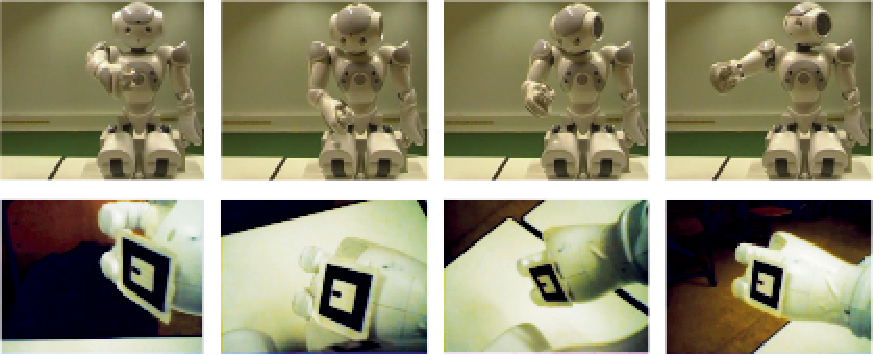
\epsfig{file=sequence.pdf, height=5cm}
\caption{A sample sequence of random motor movements during motor babbling in a robot}
\label{lab:babbling}
\end{figure}


Several robotics studies have been inspired by the infants' behaviour of body babbling.
Exploration behaviours have been implemented in artificial agents for gathering 
evidence to form internal models of their bodily characteristics 
\citep{SchillaciHLG13, Saegusa2009}.
Schillaci et al. propose a way for combining knowledge through exploration and 
knowledge from others \citep{SchillaciHLG13}, and Demiris et al. use mirror 
neuron inspired internal models \citep{Demiris2005}.
An exploration mechanism driven by the active 
self-generation of high-level goals has been proposed by Baranes 
\citep{baranes2013}. Such a mechanism allows active learning of inverse models 
in high-dimensional redundant robots. 

In this thesis acquisition of coordination skills through random 
motor babbling has been implemented on a humanoid robot Nao from Aldebaran. 
Physical dimensions of the Nao resemble those of a child standing at a height of 
ca. 57 cm and simulating the real visual input perceived by a young human 
subject. A sample babbling sequence is shown in Figure \ref{lab:babbling} where 
the first row shows random hand movements, and the second row the corresponding 
frames captured by the camera. The implementation of the babbling procedure was 
adapted from \citep{SchillaciH11}. The robot has been provided with a simple 
behaviour based on sensorimotor coordination which allowed it to look at its own 
random arm movements. In particular, the behaviour consisted of the following 
steps: a motor command, that is, a desired angle position, is sent to each joint 
of the arm (only one arm is babbling); when the hand of the robot, represented 
for simplicity by a marker\footnote{We used the ARToolkit library for marker 
detection (http://www.hitl.
washington.
edu/artoolkit).}, is detected, the joints of the neck are rotated in order to center the marker in the perceived visual input. 
The bottom camera placed in the robot's head has been used to capture the visual input at a varying speed between 9 and 30 frames per second.
During the babbling process, information related to the estimated position of the marker is stored and mapped with the current configuration of the arm joints in a knowledge base. 
The position of the marker is characterised by a horizontal, vertical and depth dimension. The depth dimension is computed based on the dimensions of a marker provided through a configuration file to the ARToolkit library.
Four arm joints have been used: shoulder pitch, shoulder roll, elbow yaw and elbow roll. 
%Together, the marker position and positions of joints form a 7D data point. 

By implementing the random motor babbling algorithm on a robot we make several assumptions regarding the development of sensorimotor skills. First, we assumed that the ``hand regard'' behaviour is already learned since the robot is able to gaze at its moving hand. By equipping the robot with a system for marker detection, we shortcuted a part of the developmental trajectory which is known to exist in infants. 
In \citep{Metta2000} this stage of the development has also been learned, in addition to acquisition of numerous other sensorimotor skills.
Second, there exists evidence for goal babbling \citep{rolfs2012}, stating that infants already few days after birth try to reach goals, although they constantly fail. Using a random walk strategy we excluded the role of goal-directed behaviours. We made these assumptions because this thesis does not concern itself with the extent to which sensorimotor skills are innate or learned.

\section{The SOM-based Model}
\label{sec:themodel}

We aim to develop a model for coding sensorimotor experience inspired by computational properties of sensory maps in the human brain (section \ref{ssec:braindev}). In particular, we phenomenologically simulate experience-dependent plasticity in the model based on the robot's interaction with the environment. In the human brain, sensory maps contain neurons specialised in processing of information coming from specific sensory modalities. Our model is motivated by two characteristics of sensory maps: topological structure and the self-organising property. 

\subsection{Simulating Sensory Maps}
\label{sec:simsensmaps}

Sensory maps can be simulated using artificial neural networks (ANNs), which are 
computational algorithms inspired by the brain organisation and structure. 
Expressed using mathematical vocabulary, an ANN is a graph whose nodes are 
neurons organised in a layered architecture and connecting edges among them are 
neural weights. Weights are computed using various learning rules such as 
backpropagation algorithm or gradient descent. Resulting weights accomplish 
mapping of the input values to the desired outputs by approximating an initially 
unknown function which describes that relation.
In the mathematical theory of neural networks, they are called universal function approximators (for mathematically rigorous description see \citep{Kurt1991251}).
ANNs do not capture the exhaustive level of information processing detail as observed in real biological systems. They rather attempt to reproduce experimental data by taking the same stimulus as input, or are used to computationally reproduce phenomena observed in neural systems. 

Based on insights into the way the brain represents and manipulates sensory information presented in section \ref{sec:neurosci}, we decided to a use a particular class of ANNs known as \emph{self-organising maps} (SOMs) or Kohonen networks \citep{Kohonen}. 
SOMs have been widely utilised in modelling of formations of different sensory modalities such as those in the auditory cortex \citep{MartinezRitterSchulten1988}, somatotopic maps \citep{Obermayer:1990} and orientation maps in the striate cortex \citep{malsburg73}.
Also, SOMs are well suited for learning hand eye-coordination without a priori model of arm kinematics in the simulated \citep{Marggie94} as well as the physical \citep{Martinetz} robotic arm. 
One of the reasons for using a biologically-inspired model is to gain better 
understanding of the biological system through computational modelling. We use a 
brain-inspired Hebbian learning paradigm to associate maps to simulate 
interaction between brain areas based on the interaction of the agent with the 
external world.
 
In \citep{Kohonen} an explanation is provided that states the relation between formalisms behind SOMs and physical or neural systems. In another words, it is possible to express biological processes or mechanisms in terms of mathematical formulas or algorithms. Two relations between SOMs and neural systems are identified which can be studied independently: formation of an activity cluster around the neuron with the maximal activity (1) and the adaptive change in the input weights of those neurons where activity was confined (2). The phase (1) is supported by the anatomical and physiological evidence for lateral interaction between neural cells: short-range excitation and long-range inhibition (Figure \ref{fig:interact} (a)). A schematic representation of a network  which may implement such a function is shown in Figure \ref{fig:interact} (b). The phase (2) is related to limited synaptic resources such as 
neurotransmitters and energy, and the change of synaptic efficacy depending on the type and location of the synapse.



\begin{figure}[t]
\centering
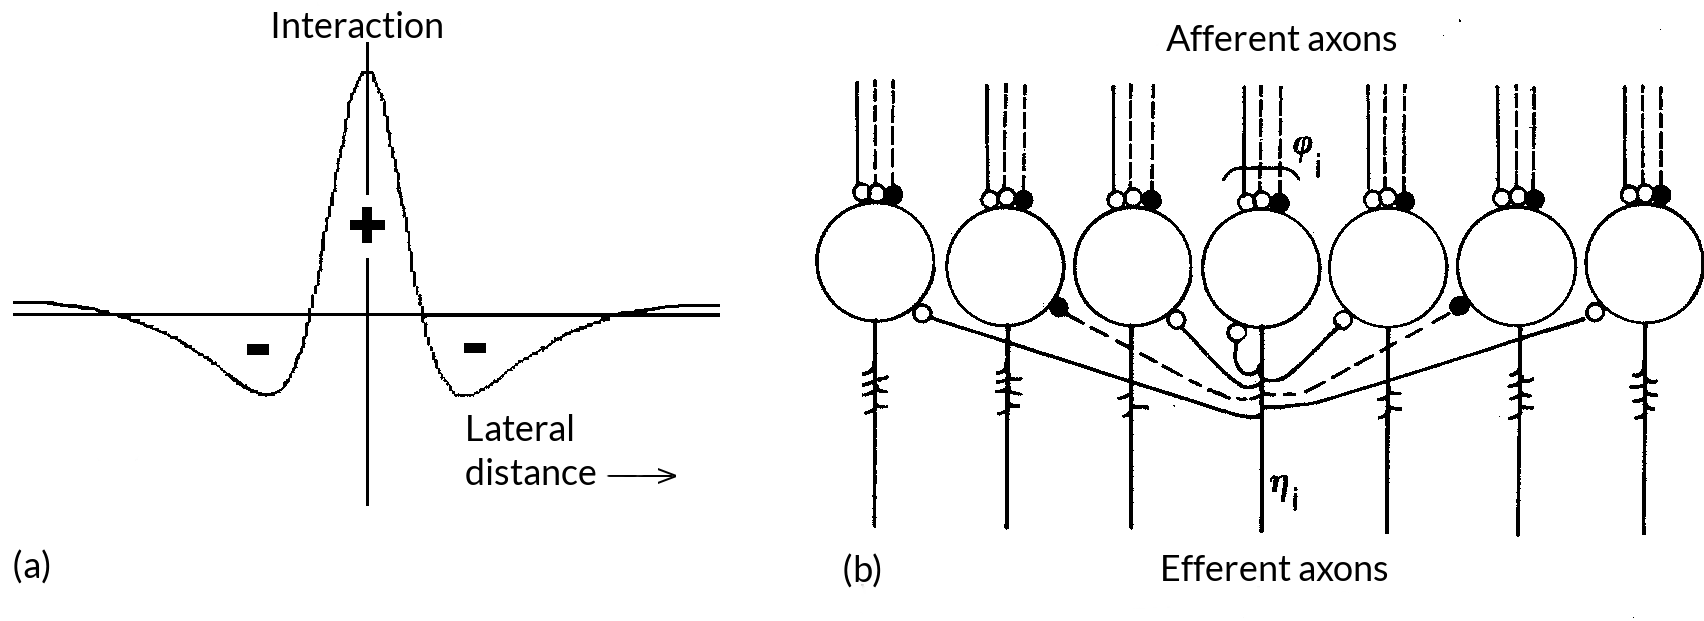
\includegraphics[scale=0.25]{soms_bio_hor.png}
%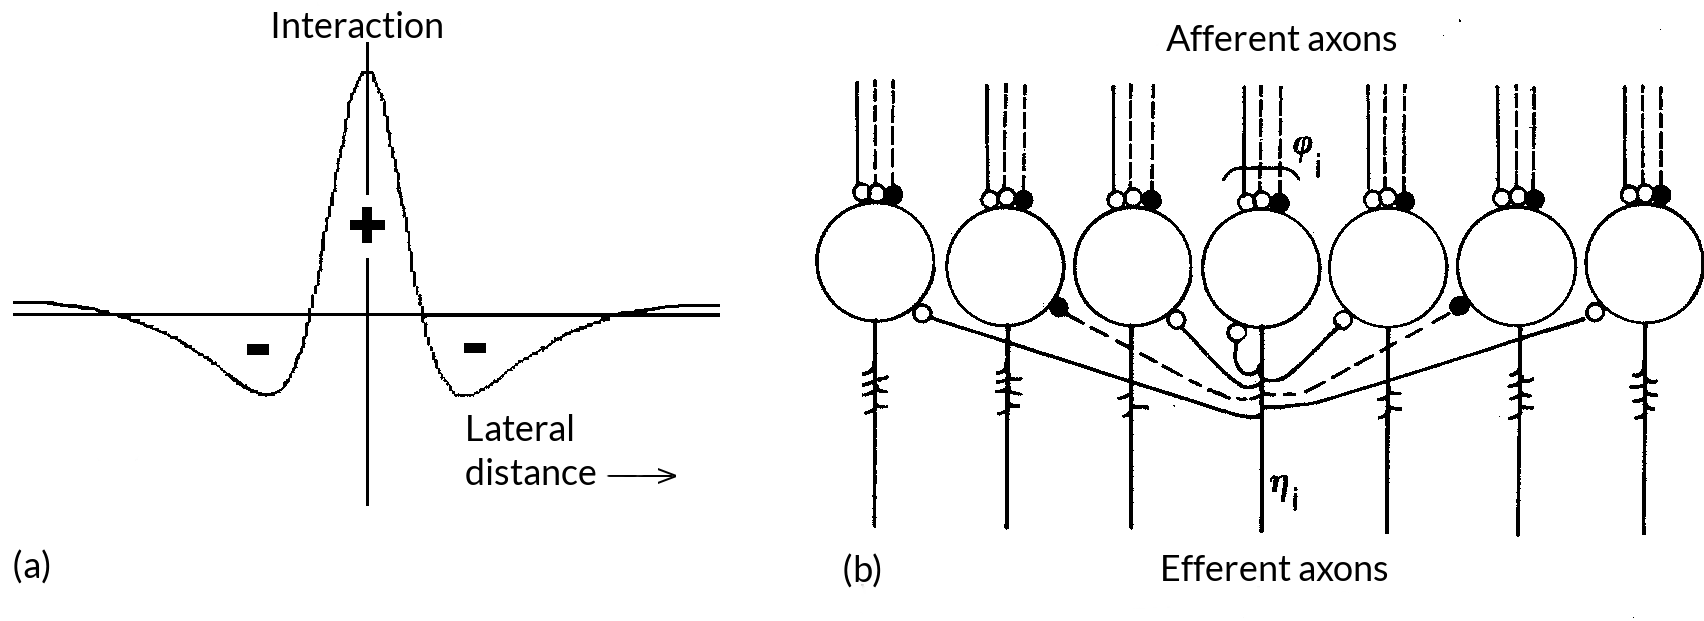
\epsfig{file=soms_bio_hor.png, height=5.5cm}
\caption[Lateral connectivity around the winning neuron in a SOM]{Profile of the function describing the interaction of the winning neuron and neighbouring neurons (a) and schematic representation of lateral connectivity which may implement that function (b) (Figure adapted from \citep{Kohonen})}
\label{fig:interact}
\end{figure}



\subsection{Formalisms behind SOMs}
\label{sec:sommath}


A SOM is constructed as a grid of neurons, where each neuron is represented as 
an $n$-dimensional weight vector $\mathbf{w_i}$. Neigbouring neurons are 
connected in a topological structure.
The number of dimensions of a weight vector corresponds to the dimensionality of input data. Each neuron approximates a certain region of data points in the input space yielding less units needed to represent the input. For this reason, one often refers to SOMs in terms of dimensionality reduction algorithm which is not to be confused with algorithms such as PCA, SFA or ICA which aim to find the low-dimensional representation of the input.

Weights in the network are initially set to random values and then adjusted iteratively by presenting the input vector $\mathbf{x_p}$ which is randomly chosen from the input data. In each iteration, the winning neuron $i$ is selected as a neuron whose weights are closest to the input vector in terms of the Euclidean distance:
\begin{equation}
\underset{i}{\arg\min} || \mathbf{x_p}-\mathbf{w_i} ||
\end{equation}
After selecting a winning neuron, the weights of all other neurons, here denoted as $j$, are adjusted:
\begin{equation}
\mathbf{\Delta w_{j}} = \eta(t) h(i, j) (\mathbf{w_{j}}-\mathbf{x_p})
\end{equation}

The $\eta(t)$ parameter is a learning rate which defines the rate at which the weights are changed.
The function $h(i, j)$ is a Gaussian neighborhood function defined over the grid of neurons as:
\begin{equation}
%h(i, j)=e^{(\frac{\mathbf{w_i^2}-\mathbf{w_j^2}}{2\pi\sigma(t)^2})}
h(i, j)=e^{-\left(\frac{\mathbf{w_i^2}-\mathbf{w_j^2}}{2\pi\sigma(t)^2}\right)}
\end{equation}

The profile of the Gaussian neighborhood function is inspired by the lateral connectivity profile as shown in Figure \ref{fig:interact} (a). The function is centered around the winning neuron $i$ and its values are computed for all neurons $j$ in the grid.
 The spread of the function determines the extent to which neighbouring weights of a winning neuron are going to be affected in the current iteration. The topology of the network is preserved by pulling together neurons closest to the winning node.  
The learning rate $\eta$ and the spread of the Gaussian function $\sigma$ are held constant for the first half of iterations, and afterwards are annealed exponentially. This underlies the assumption that the initial configuration of neurons in the network poorly covers the space, and only upon iterative presentations of input data starts converging to the optimal state.

The activation function of a neuron, $A(\mathbf{x})$ is computed over the Euclidian distance ($\textbf{x}$) between the neural weights and the input vector:
\begin{equation}
A(\mathbf{x}) = \frac{1}{1+\tanh(\mathbf{x})}
\end{equation}

It is a common practice in cognitive modelling to connect multiple SOMs using the associative links \citep{Morse2010}, \citep{Westerman02modellingthe} and \citep{COGS:COGS716}. The Hebbian learning paradigm describes an associative connection between activities of two connected neurons. If a postsynaptic neuron $j$ is always activated after the presynaptic neuron $i$, the connection between these two neurons is strengthened using the following rule:
\begin{equation}
\Delta w_{ij} = \eta_h A(\mathbf{x_i}) A(\mathbf{x_j})
\end{equation}

Vectors $\mathbf{x_i}$ and $\mathbf{x_j}$ are distances between winning neurons and the corresponding inputs in two different maps.
Initially, all weights between two SOMs are set to zero allowing for an activity-dependent role of structural growth in neural networks.


\subsection{Model Architecture}

The inspiration for the model architecture comes from the Epigenetic Robotic 
Architecture (EPA) which was proposed as a framework for guiding modelling 
efforts \citep{Morse2010}. The basic ERA unit consists of SOMs connected via 
Hebbian weights to a central SOM acting as a ``hub''. Depending on the use case, 
different ERA units can be associated to different brain regions depending on 
the type of information they represent or the type of processing. For example, 
maps are used to represent different physical features such as the color space, 
the body posture and the word space. The architecture is implemented on a 
humanoid robot iCub and is capable of reproducing a wide range of psychological 
phenomena with results comparable to those obtained in experiments with humans. 
It is not tailored to specific domains or tasks, making it suitable for 
extensions and novel applications. In addition, it displays an ongoing 
developmental trajectory providing a ground to analyse learning behaviours of 
agents 
interacting with the environment.

Based on guiding lines provided by the ERA, we decide to associate two 2D SOMs.
Each SOM represents a different part of the left arm posture. Neurons in each SOM are ordered in a grid consisting of rows and columns, such that each neuron is identified by a 2D index. This is schematically depicted in Figure \ref{lab:model} where the ``blue'' SOM is used to represent the elbow and shoulder positions, and the ``red'' SOM the hand positions. Every neuron in the ``blue'' SOM is identified through a 3D weight vector ($x, y, z$), and every neuron in the ``red'' SOM through a 4D weight vector ($\sigma_p, \sigma_r, \epsilon_y, \epsilon_r$). The weights of neurons in the first SOM are meant to represent vertical, horizontal and depth dimensions, while weights in the second SOM stand for shoulder pitch, shoulder roll, elbow yaw and elbow roll. Those weight are later used when issuing a motor command to the robotic arm.
Arrows in the figure depict Hebbian weights, such that thicker arrows represent stronger synaptic connections. Different instances of a model are named according to the number of neurons in each row and each column in a single SOM (e.g. \ssom model or \bsom model). 

\begin{figure}[t]
\centering
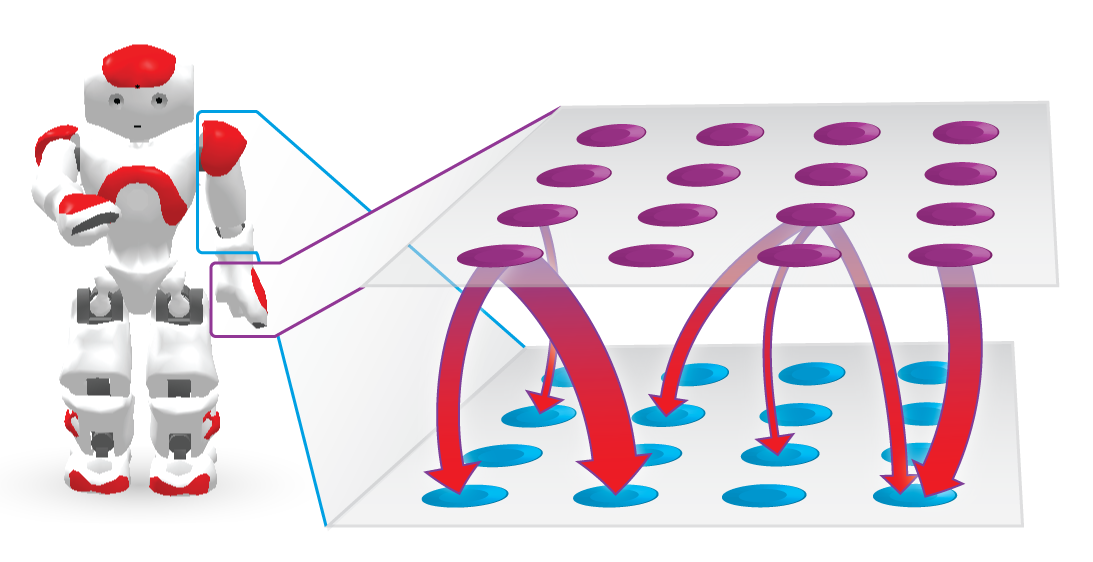
\epsfig{file=model.png, height=6cm}
\caption{Scheme of the model architecture for learning hand-eye coordination with SOMs and connecting weights}
\label{lab:model}
\end{figure}

\section{Training Data}
\label{sec:modeltrain}

The weights of neurons were adjusted using the data obtained in the babbling experiment. 
From the knowledge base constructed in the babbling experiment, two training sets were created. One training set comprised of the 3D hand coordinates and the other of 4D joint coordinates.


